%%%%%%%%%%%%%%%%%%%%%%%%%%%%%%%%%%%%%%%%%%%%%%%%%%%%%%%%%%%%%%%%%%%%%%%%%%%%%%%%
%2345678901234567890123456789012345678901234567890123456789012345678901234567890
%        1         2         3         4         5         6         7         8

\documentclass[preprint,5p]{elsarticle}

\usepackage[utf8x]{inputenc}
\usepackage[T1]{fontenc}

\usepackage[english]{babel}
\usepackage{cite}
\usepackage{graphicx, subfigure}
\usepackage{url}
\graphicspath{{figs/}}
\DeclareGraphicsExtensions{.pdf,.jpg,.png}

\usepackage[draft, nomargin, marginclue, footnote]{fixme}

\usepackage{listings}
\usepackage{alltt}
\usepackage{fancyvrb}

%\usepackage[bookmarks]{hyperref}

\newcommand{\concept}[1]{{\small \texttt{#1}}}

\newcommand{\stmt}[1]{{\footnotesize \tt $\langle$ #1\relax$\rangle$}}

\newcommand{\ie}{{\textit{i.e.\ }}}
\newcommand{\cf}{{\textit{cf\ }}}
\newcommand{\eg}{{\textit{e.g.\ }}}

\begin{frontmatter}

\title{\LARGE \bf
Human-Robot Interaction: A Deliberative Architecture
}

\author{Rachid Alami, Séverin Lemaignan, Aurélie Clodic, Mathieu Warnier}

\address{
CNRS, LAAS, 7 avenue du Colonel Roche, F-31400 Toulouse, France\\
Univ de Toulouse, LAAS, F-31400 Toulouse, France\\
{\tt firstname.lastname@laas.fr}
}




%%%%%%%%%%%%%%%%%%%%%%%%%%%%%%%%%%%%%%%%%%%%%%%%%%%%%%%%%%%%%%%%%%%%%%%%%%%%%%%%
\begin{document}
\begin{abstract}

This paper addresses some key decisional issues that are necessary for a
cognitive robot which shares space and tasks with a human. We adopt a
constructive approach based on the identification and the effective
implementation of individual and collaborative skills. The system is
comprehensive since it aims at dealing with a complete set of abilities
articulated so that the robot controller is effectively able to conduct in a
flexible manner a collaborative task with a human partner. These abilities
include geometric reasoning and situation assessment based essentially on
perspective-taking and affordances, management and exploitation of each agent
(human and robot) knowledge in separate cognitive models, human-aware task
planning, and human and robot interleaved plan achievement.

This article presents our design choices, the articulations between the diverse
deliberative components of the robot, and the strengths and weaknesses of our
approach. We show that explicit knowledge management is not only a convenient
tool from the software engineering point of view, but also pushes for a
different, more \emph{semantic} way to address the decision-making issue in
human-robot interactions.

\end{abstract}

\begin{keyword}
    %% keywords here, in the form: keyword \sep keyword
    human-robot interaction \sep cognitive robotics \sep perspective taking \sep knowledge representation and reasoning
    %% MSC codes here, in the form: \MSC code \sep code
    %% or \MSC[2008] code \sep code (2000 is the default)

\end{keyword}

\end{frontmatter}

\listoffixmes

%%%%%%%%%%%%%%%%%%%%%%%%%%%%%%%%%%%%%%%%%%%%%%%%%%%%%%%%%%%%%%%%%%%%%%%%%%%%%%%%

\section{The challenge of human-robot interaction}

Human-robot interaction is a challenge for artificial intelligence. This field
indeed lays at the crossroad of several other domains of AI and requires to
tackle them in a holistic manner. Modeling humans and human cognition;
acquiring, representing, manipulating in a tractable way abstract knowledge;
reasoning on this knowledge to make decisions; instanciating those decisions
into physical actions in coordination with humans... Many AI techniques are
invited, from visual processing to symbolic reasoning, from task planing to
\emph{theory of mind} building, from reactive control to action recognition and
learning.

We do not tackle all these issues. This article attempts however to organize
them into a coherent challenge for artifical intelligence, and also explicit
some of the trails that have been explored on our robots and that result in a
deliberative, knowledge-focused, architecture for human-robot interaction.

Human-robot interaction requires to equip the robot with explicit reasoning on
the human and on its own capacities to achieve its tasks in a legible, if not
collaborative, way with human partners. In the following pages, we present a
robot control system which has been especially designed for a cognitive robot
which shares space and task with a human. It has been designed by adopting a
constructive approach based on effective individual and collaborative skills.
The system is comprehensive since it aims\fxnote{it *is* comprehensive, or it *aims* at being comprehensive?} at dealing with a complete set of
abilities articulated so that the robot controller is effectively able to
conduct in a flexible manner a collaborative task with a human partner.

We illustrate below how we deal with a typical human-robot interactive task
achievement and what are the abilities we claim are necessary. Section
\ref{sec:problem} proposes a typical human-robot interaction problem that can
be solved by the proposed robot controller. Section
\ref{sec:Framework} provides an overview of the robot controller and
introduces three activities which are described in \ref{sec:situ},
\ref{sec:plan} and \ref{sec:action}. Section \ref{sec:expes}
presents the structure an actual run on a real robot in face to face interaction with a
person. Finally, section~\ref{sec:soa} discusses and analyses the impact of
each of our contribution in the light of existing literature and alternative
approaches.

\subsection{The human-robot interaction challenge}\label{sec:problem}

\fxfatal{Develop/reorganize this section to organize the different problems of
HRI into one coherent challenge for AI. See how to articulate it with section
\ref{sec:psychocognitivegrounds}}

We envision HRI in a context where two agents (a human and a robot)
share a common space and exchange information through various
modalities. Our aim is to endow the robot with an explicit
consideration of the human and with the ability to manage its
interactions with him (Figure~\ref{fig:hri-dec}). This must be
considered at the architecture level as well as at the task/motion
planning and execution level. 

\begin{figure}[htb]
\centering
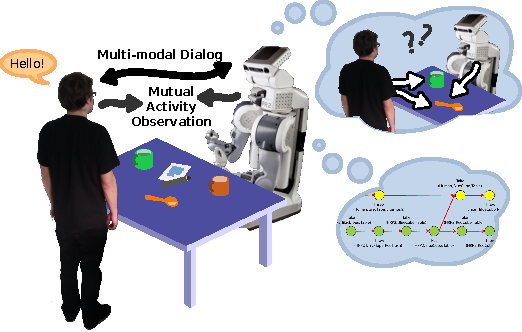
\includegraphics[width=0.9\columnwidth]{figs/grounding_robot.pdf}
\caption{Robot reasoning about HRI and anticipation of human activities:
  sources of information are multi-modal dialogue, and observation of
  environment and human activity}
\label{fig:hri-dec}
\end{figure}

\paragraph{The Joint Action Challenge} Let us consider a robot which is
supposed to achieve interactive object manipulation, fetch and carry tasks and
similar tasks in a domestic environment. The problem we are dealing with here
is the following. Given:

\begin {itemize}
\item a joint goal, which has been previously established and agreed
  upon (through a process which is out of the scope of this paper),
\item the current situation, acquired through perception or
  deduction from previous perceptions, including the state of the
  environment of the robot and of the human,
\end {itemize}

the robot controller computes an action to execute and who (the 
human or the robot, or both in case of a joint action) has to perform
it, and then controls or monitors its execution. The operation
continues until the goal is achieved, is declared unachievable or is
abandoned by the human.

To do so, the robot has to be equipped with a number of decisional, planning
and interpretation abilities where its human partner is taken
explicitly into account. It needs to be able:

\begin {itemize}
\item to build and maintain relevant robot and human beliefs
  (from the robot perspective) with respect to state of the world and the task,
\item to build and maintain iteratively shared (human-robot) plans, 
\item to refine and execute the actions it has to perform, and to monitor 
those achieved by its human partner.
\end {itemize}

Besides, we would like to build such abilities in a generic way, and
to provide several levels of parametrization allowing to adapt to
various environments, and various levels of involvement of the robot
ranging from teammate behavior to assistant or proactive helper.

We have devised a decisional framework for human-robot interactive
task achievement that is aimed to allow the robot not only to
accomplish its tasks but also to produce behaviors that support its
engagement vis-a-vis its human partner and to interpret human
behaviors and intentions. 
Together and in coherence with this framework, we have developed
and experimented various task planners and interaction schemes that
allow the robot to select and perform its tasks while taking into
account explicitly the human abilities as well as the constraints
imposed by the presence of humans, their needs and preferences. 



\subsection{Our Contributions Towards the Cognitive Robot}

The main scientific contributions of the article are summarized here, to guide
the reader. We develop and discuss them, also in relation to other works, at
the end of the article.

\fxfatal{Rewrite section 'summary of contributions'}

Over the last years we have focused our efforts on identifying the cognitive
prerequisites of these challenges, and giving them experimental reality on the
robots: what is required for sentences like ``Let's set the table together''
to be understood by the robot, correctly interpreted in the spatial and
temporal context of the interaction, and eventually transformed into a set of
actions.

We have chosen to tackle the challenge from several ends: human-aware
navigation and motion planning~\cite{Mainprice2011}, situation assessment
coupled with motion planning~\cite{Mainprice2012}, projection of
``mightabilities'' that anticipates what surrounding agents may
do~\cite{Pandey2011}, and the design and deployment of a pervasive
\emph{knowledge-oriented} software architecture~\cite{Lemaignan2013}.

\section{From Human-Robot Interaction to a Deliberative Architecture}

\subsection{The Psycho-Cognitive Grounds of Human-Robot Interaction}
\label{sec:psychocognitivegrounds}

\fxfatal{write section summary of the challenges that human-robot interaction presents to robotics.}

\subsection{Building a human-aware deliberative layer}

\fxfatal{Need to carefully introduce this section: how did we come up this this architecture?}

Fig.~\ref{fig|archi} gives an overview of the connections between the
deliberative components of our architecture~\cite{Alami2011}.

\begin{figure*}
        \centering
        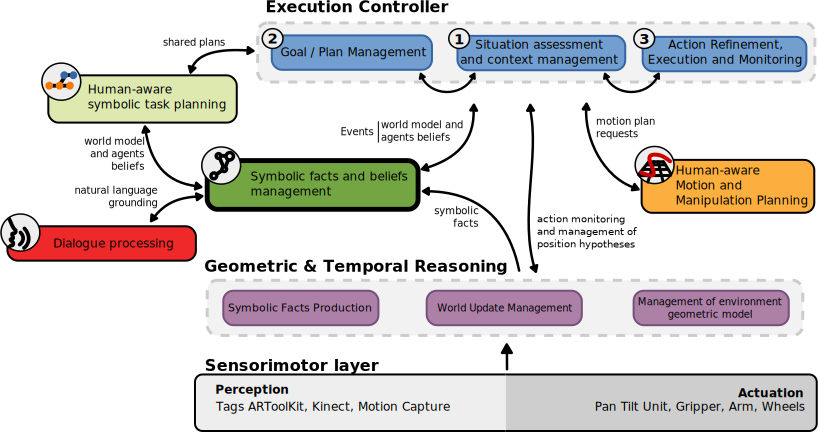
\includegraphics[width=1.0\columnwidth]{archi}
        \caption{Overview of the LAAS deliberative layer. Knowledge is
        centrally managed in an active \emph{semantic blackboard}, pictured
        above with a thick border.}
        \label{fig|archi}
\end{figure*}


This architecture moves away from standard layered approaches. Interactions
between components at the deliberative level are mostly bidirectional and we do
not introduce layers of abstraction amongst software components\footnote{We do
have lower-level modules to execute actions or manage sensors, but all
cognition-related modules reside at the same level.}. This is nicely
illustrated by the dialogue input processing. This component does not simply
act as an alternative perceptual input to the symbolic database; it also
actively queries previously acquired knowledge to disambiguate and validate the
newly created symbolic knowledge (see section~\ref{sect|com}).

Our architecture relates to \emph{Beliefs, Desires, Intentions} (BDI)
architectures. BDI architectures are primarily focused on \emph{practical
reasoning}, \ie the process of deciding, step by step, which action to perform
to reach a goal (as summarized by Woolridge~\cite{Woolridge1999}). The
management of the interaction between knowledge (the beliefs) and task and plan
representation and execution (the desires and the intentions) is central, and
aims at selecting at each step the best subgoal. It becomes then an intention
that the robot commits to.

This interaction between knowledge and actions is also central to our approach
(as for any cognitive system): it is one of the activities of the
robot, actually shared between communication components (that can acquire
desires from interaction with agents, amongst other things) and an execution
controller that may decide to take an incoming desire into account to create
its own internal goals. The controller generates and manages intentions from
these goals with the help of a symbolic task planner, that also has direct
access to the knowledge base.

This activity is however not the backbone of our architecture. Other
activities are conducted in parallel, without being explicitly considered as
desires: assessment of the situation and the environment, dialogue (including
performative dialogue that can possibly change the internal state of the robot,
but does not lead to the creation of desires, like question answering or
statement assertion), various background monitoring and recognition tasks, etc.

Regarding the anchoring question, this architecture is bidirectional. The
components we described provide a \textit{bottom-up} grounding process:
geometric reasoning and dialogue processing modules constantly build and push
new symbolic contents about the world to the knowledge base where it becomes
accessible to decisional layers. In parallel, the knowledge base relies on
reasoning in a \textit{top-down} way to produce new facts that may in return
trigger physical behaviours.

\subsection{A Knowledge model}

In our architecture (Fig.~\ref{fig|archi}), knowledge manipulation relies on a
\emph{semantic blackboard}: a central server (the {\sc Oro}
server~\cite{Lemaignan2010}) stores knowledge as it is produced by each of the
deliberative components. It conversely exposes a {\tt json}-based RPC API to
query the knowledge base~\cite{lemaignan2012kbapi}.

Knowledge is represented as RDF triples in the OWL sub-language. Each
time triples are added or removed from the knowledge base, a Description
Logics reasoner ({\sc Pellet}\footnote{\url{http://clarkparsia.com/pellet/}})
classifies the whole ontology and inserts all possible inferred triples.

Relying on RDF triples and Description Logics has advantages such as the
availability of numerous mature open-source libraries to manipulate the ontology,
interoperability with several major on-line knowledge bases (like {\sc
OpenCyc}, {\sc WordNet} or {\sc DBPedia}), open-world reasoning, and the formal
guarantee of decidability (it is always possible to classify a Description
Logics ontology).

It also has notable limitations, both fundamental (the suitability
of Description Logics when reasoning on --typically non-monotonic-- commonsense
knowledge is questionable) and practical: RDF triples imply only binary predicates
(\stmt{subject predicate object}), which constrains the expressiveness of the
system or leads to cumbersome reifications. Alternatives exist (like {\sc
KnowRob}~\cite{Tenorth2009a}) that mix RDF with more expressive logic
languages like {\sc Prolog}, at the price, however, of other limitations, like
closed-world reasoning or immutable T-Box. The classification
performance is another issue: from our experience, with an ontology sized for a
standard experiment (about 100 classes and 200 instances), classification
typically takes about 100ms, which becomes problematic during interactions.
Besides, the performances are difficult to predict, since a seemingly
inoffensive new statement may indirectly change radically the logical
complexity of the whole knowledge model and lead to notable degradation of
classification time.

This knowledge model also largely excludes representation of continuous
phenomena (like time) or uncertain phenomena. When required (for instance for
action recognition), these are managed inside the corresponding components, and
are not exposed at the semantic level.

Tools to manipulate and reason over ontologies are readily available, mature,
and already well accepted in the robotic community~\cite{Tenorth2009a,
Lim2011}. While alternatives like \emph{Answer Set Programming} have also been
successfully investigated in robotics~\cite{Chen2010,Erdem2012}, in particular
to deal with non-monotonic reasoning, we did not actually hit any brick wall
while working with OWL ontologies. We may reconsider this choice at a later
stage, but until now it has proven an effective framework to quickly explore
implementations of new cognitive abilities (for instance, it has been
conceptually and technically easy to add support for independent knowledge
models, one per the agents the robot interacts with --see
section~\ref{sect|tom}).

Besides, because ontologies and RDF statements are relatively simple concepts
to grasp, it also effectively helped to grow awareness amongst colleagues on
the significance of the ``semantic level'' when developing new components for
the robot.

\subsection{Internal cognitive processes}
\label{sect|intern}

\subsubsection{Theory of Mind}
\label{sect|tom}

Theory of Mind (originally defined in~\cite{Premack1978}) is the cognitive
ability that a subject possesses to represent the mental state of another
agent, possibly including knowledge that contradicts the subject's own model: for
example, a book can be at the same time \emph{visible} for myself, and \emph{not
visible} for you.

Children develop this skill, which is essential to understand others' perspectives during
interactions, around the age of three. It supposes the
ability to build, store and retrieve separate models of the knowledge of the
interactors.

Our knowledge base implements such a mechanism: when the robots infers a new
agent has been introduced in the knowledge base, it initializes a new,
independent, ontology for this agent. All the ontologies that are created share
the same common-sense knowledge, but rely on each agent's perspective for the
actual instantiation: the robot (geometrically) computes that the book is in
its own field of view, but not in the human one. The robot knowledge contains
the fact \stmt{book isVisible true} while the human model contains \stmt{book
isVisible false}.

One classical application of this cognitive skill is the so-called
\emph{False-Belief} experiment (also known as the \emph{Sally and Ann}
experiment)~\cite{Leslie2000}: a child is asked to watch a scene where two
people, A and B, manipulate objects. Then A leaves and B hides away one
object. When A comes back, we ask the child ``where do you think A will
look for the object?''. Before acquiring a theory of mind, children are not
able to separate their own (true) model of the world (where they know that
the object was hidden) from the model of A, which contains \emph{false
beliefs} on the world (A still thinks the object is at its original
position since he did not see B hiding it). Using separate knowledge models
in the knowledge base, we have been able to replicate this experience with
our robots~\cite{Warnier2012a}.

\subsubsection{Working memory}

The {\sc Oro} server also features a mechanism to mimic minimalistic forms of
biological memory.  When new statements are inserted in the knowledge base, a
\emph{memory profile} is optionally attached to them.

Three such profiles are predefined: {\tt short term}, {\tt episodic} and {\tt
long term}. They each correspond to a different lifetime for the statements
(respectively 10 seconds, 5 minutes and no time limit). After this duration,
the statements are automatically removed from the knowledge base.

This approach is limited. In particular, \emph{episodic} memory primarily
refers to the semantics of the statements (that is expected to be related to an
event) and not to a specific life duration.

We rely however on this short term memory for a particular use-case:
\emph{active concepts}. Some modules, like the natural language processor, use
the {\tt short term} memory profile to mark for a few seconds important
concepts that are currently manipulated by the robot. For example, if a human
asks the robot: ``Give me all red objects'', the human, the \concept{Give}
action, and each red objects that are found are successively marked as
\emph{active concepts} by inserting statements such as \stmt{human type
ActiveConcept} in the short-term memory (which can be considered, in this case,
to be a working memory). We use this feature to trace certain knowledge-related
processes.


%%%%%%%%%%%%%%%%%%%%%%%%%%%%%%%%%%%%%%%%%%%%%%%%%%%%%%%%%%%%%%%%%%%%%%%%%%%%%%%%
\section{Implementing the Cognitive Skills}

Previous section provided an overview of what we propose as a generic cognitive
architecture for robots involved in interactions with other social agents.

We now introduce each of the components and try to give insights on their main
features.


\subsection{Situation Assessment, Human Awareness, Perspective Taking}
\label{sect|sit-ass}

\begin{figure}
        \centering
        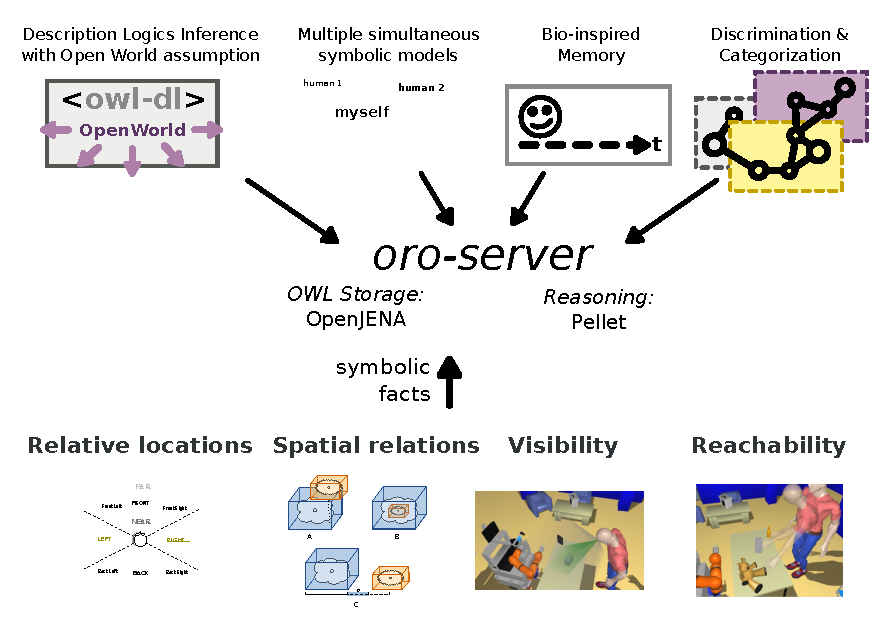
\includegraphics[width=\columnwidth]{spark-oro}
    \caption{Functional overview of knowledge base ({\sc Oro} server, top part) and the geometric situation assessment module (\emph{SPARK}, bottom part)}
        \label{fig|spark-oro}
\end{figure}

Anchoring perceptions in a symbolic model requires perception abilities and
their symbolic interpretation. We rely on a dedicated geometric and temporal
reasoning module called SPARK (\emph{SPAtial Reasoning \&
Knowledge}~\cite{Sisbot2011}). It is a situation assessment reasoner that
generates symbolic knowledge from the geometry of the environment with respect
to relations between objects, robots and humans (Fig.~\ref{fig|spark-oro}),
also taking into account the different perspective that each agent has on the
environment.

SPARK is an \emph{amodal} geometric model of the environment that serves both
as basis for the fusion of the perception modalities and as bridge with the
symbolic layer. This geometric model is continuously updated at run-time by the
robot based on its sensors (in our experiments, objects are identified and
localised through 2D barcodes, while humans are tracked with Kinect-like
devices, optionally assisted by motion capture to accurately track the head
motion, which is required to compute what the human is looking at).


\subsubsection{Situation Assessment}

\paragraph{Symbolic facts production:} 

Geometric state of the world is abstracted in symbolic facts that can
be classified in three different categories.

\begin {itemize}
\item Relative positions of object and agents, e.g.  \stmt{GREY\_TAPE
    isOn TABLE}.

\item Perception and manipulation capacity and state of agents,
  e.g. \stmt{ROBOT looksAt GREY\_TAPE}, \stmt{GREY\_TAPE isVisibleBy
    HUMAN1}.

\item Motion status for object or agent parts, e.g.  \stmt{GREY\_TAPE
    isMoving true},\\ \stmt{ROBOT\_HEAD isTurning true}.
\end {itemize} 

Reasoning about human perspective allow to compute facts such as:
\stmt{GREY\_TAPE isBehind HUMAN1}, \stmt{GREY\_TAPE isVisibleBy
  HUMAN1}.

Figure~\ref{fig::reach-ex} illustrates different situations for the
\textit{reachable} relation. In this case, the robot and its human partner
are placed face to face, in a table-top setup (Figure~\ref{fig::reach-ex}.1).
The robot first estimates if the small grey box is reachable to itself. This is
done by finding a collision free posture to reach the object
(Figure~\ref{fig::reach-ex}.2). Next the robot switches to the human's
perspective to estimate if the same object is reachable to the human as well.
In the last scene, the human moves towards his left, farther from the object
(Figure~\ref{fig::reach-ex}.4). The situation is then reevaluated. In this
occasion though, the reasoner cannot find a satisfactory posture for the human
to reach the box because he is too far from the target.

\begin{figure*}[!t]
	\centering
	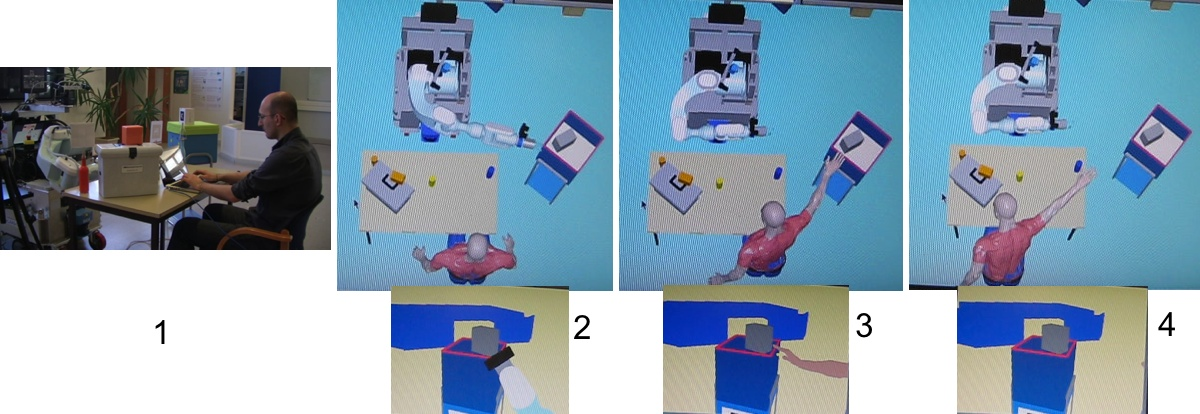
\includegraphics[width=1.0\textwidth]{figs/reachex.jpg}	
	\caption{An example illustrating the \textit{reachable} relation. The relation is computed from the perspectives of both the robot and the human. The computed posture at each step is illustrated with a global view of the scene (top), and from a closest view (bottom).}
\label{fig::reach-ex}
\end{figure*}

\begin{figure*}[ht!]
   \label{fig:sparkSubfigures}
   \begin{center}
%
       \subfigure[Initial state]{%
%           \label{fig:wuweiPhoto}
           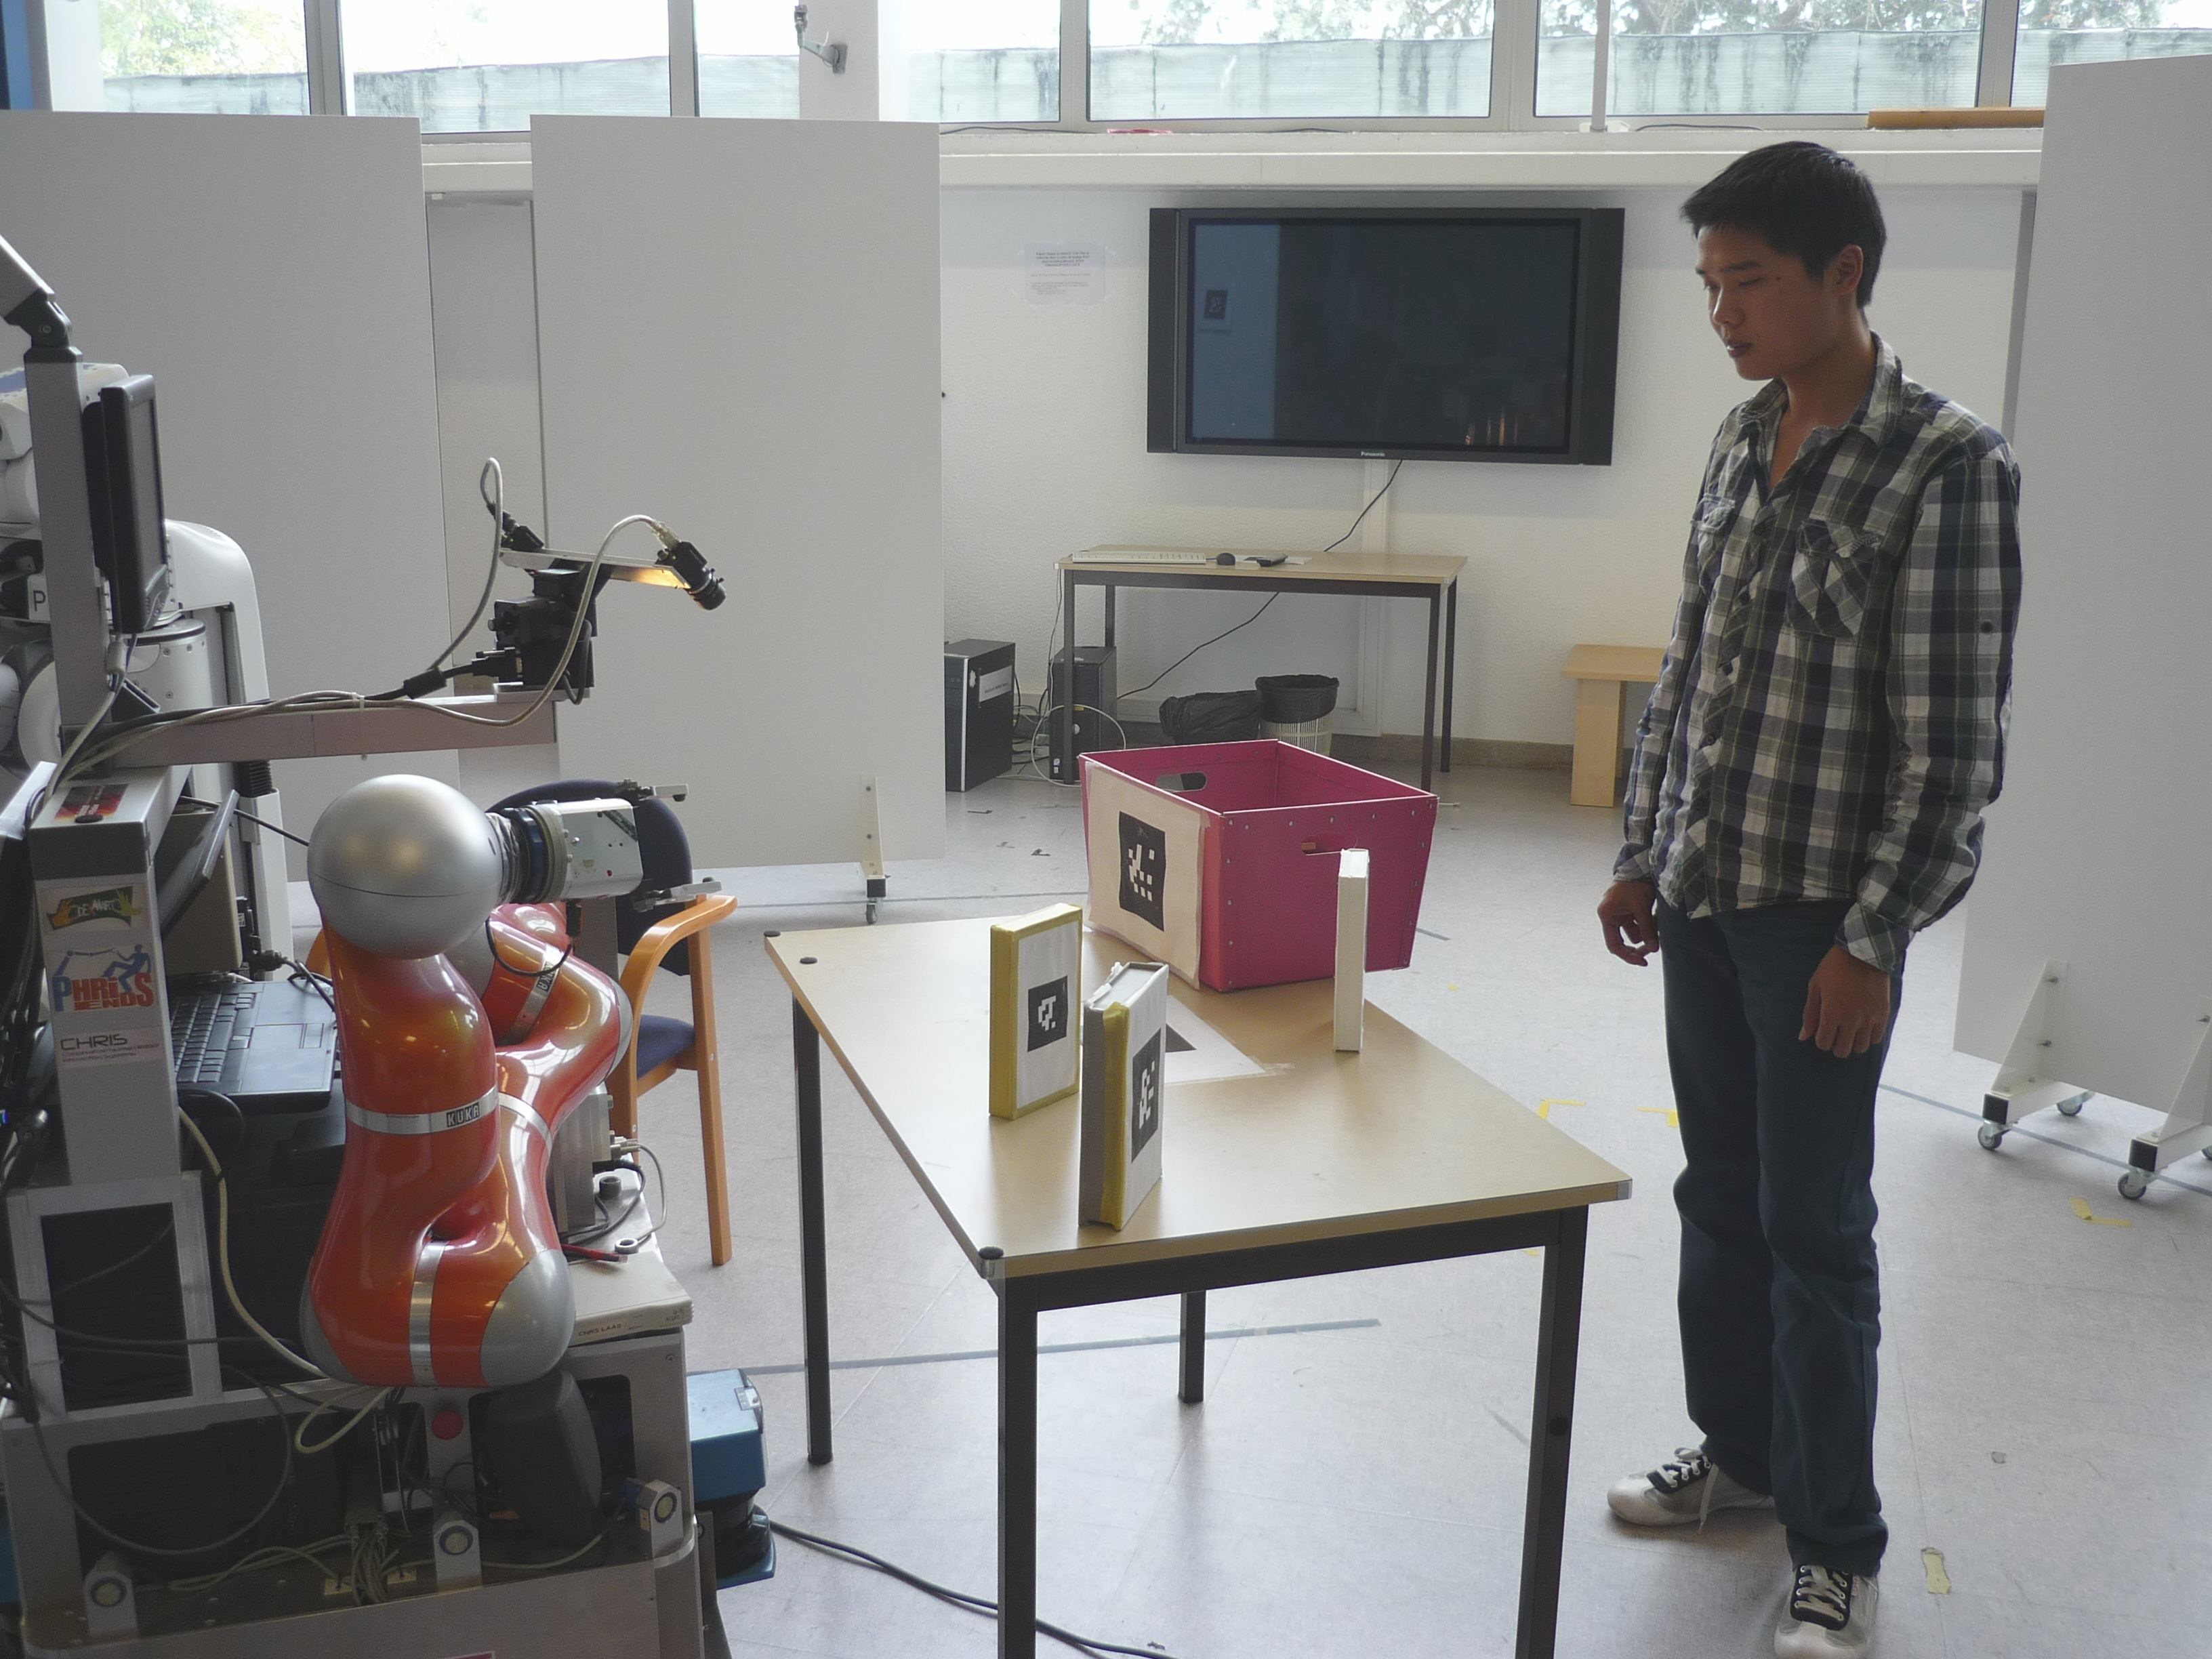
\includegraphics[width=0.5\textwidth]{./figs/etat2-P1010769_brightened-v2.jpg}
       }%
       \subfigure[3d model view of initial state]{%
%          \label{fig:sparkScreenshot}
          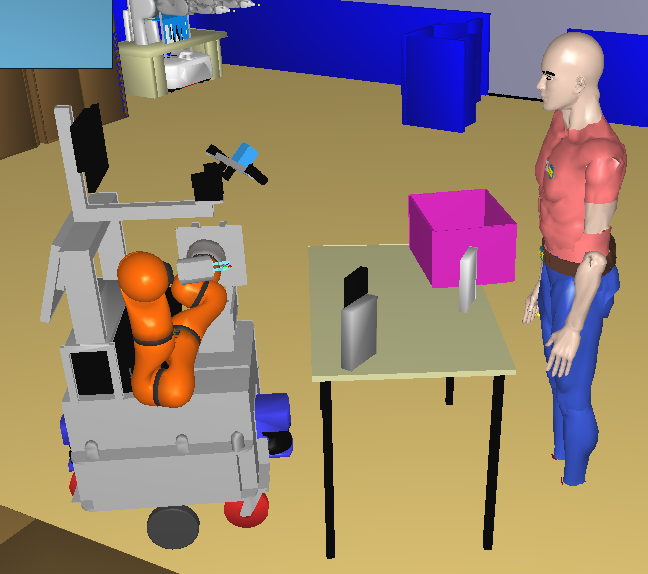
\includegraphics[width=0.43\textwidth]{./figs/etat2_photo.png}
       }\\ %  ------- End of the first row ----------------------%
%
   \end{center}

   \caption{%
     In this situation, there are three tapes on the table. Two tapes
     are only reachable by the robot: the LOTR\_TAPE (black in the 3d
     model) and GREY\_TAPE. The third tape WALLE\_TAPE (white in the
     3d model) and the trashbin PINK\_TRASHBIN are only reachable by
     the human HUMAN1. All tapes are on the table TABLE.  }%

\end{figure*}

The set of facts computed in the situation depicted by
Figure~\ref{fig:sparkSubfigures} is the following:
\begin{footnotesize}
%\begin{small}
\begin{verbatim}
                ROBOT                          HUMAN1
PINK_TRASHBIN isReachable false    PINK_TRASHBIN isReachable true 
WALLE_TAPE isReachable false       WALLE_TAPE isVisible true 
LOTR_TAPE isReachable true         LOTR_TAPE isReachable false 
GREY_TAPE isReachable true         GREY_TAPE isReachable false
WALLE_TAPE isVisible true          WALLE_TAPE isReachable true 
LOTR_TAPE isVisible true           LOTR_TAPE isVisible true 
GREY_TAPE isVisible true           GREY_TAPE isVisible true 
WALLE_TAPE isOn TABLE              WALLE_TAPE isOn TABLE 
LOTR_TAPE isOn TABLE               LOTR_TAPE isOn TABLE 
GREY_TAPE isOn TABLE               GREY_TAPE isOn TABLE 
\end{verbatim}
%\end{small}
\end{footnotesize}

\paragraph{Hypotheses on objects states and positions}
It is sometimes difficult or even impossible to see and/or track an
object in certain states. This happens, for instance, when the object
has been put in a container, when it is in the robot gripper or in the
human hand, and more generally in any state in which it is hidden by
something else. Our robot has a model of the possible symbolic states
for an object (whether the object is on a furniture, in an agent hand,
in a container, etc.).  According to the robot perception of what has
happened since the object was last seen, the robot tries to maintain a
belief of the current possible symbolic states and their associated
probabilities for this object. Such information can be used to update
the beliefs using input from exploration, dialog, human visual
focus,\ldots
SPARK currently provides a simple implementation of such a functionality. The
only managed hypotheses are \emph{in container} and \emph{in agent hand}. We
can have only one hypothesis at the same time. Hypothesis validity is checked
geometrically in case of incoming perception values.


\paragraph{Primitive action recognition}
Monitoring human activity is crucial to maintain a coherent state of
the world. Full human action and activity monitoring is a difficult
task that requires knowledge and reasoning both on high level facts
like goals, intentions and plans, as well as bottom-up data from agent
and object motions. Simple temporal and geometric reasoning on human
hand trajectories and potential objects placements can provide some
useful clues for high level human monitoring processes. We call this
temporal and geometric reasoning \emph{primitive action recognition}.

For example, a \emph{pick}, a \emph{throw} or a \emph{place} action
can be recognized by observing that an object on table and an empty
human hand are close to each other, or that the human hand holding an
object is close to a container, etc. Human hand position is either
directly perceived or inferred from its initial perceived trajectory.
We have a simple implementation of such a primitive action recognition
in SPARK that relies on monitoring human hand and its motion near
objects or above containers.


\subsubsection{Ego-centric and allo-centric frames}

SPARK enables \emph{perspective-taking}: spatial relations between entities can
be computed from different viewpoints, which let the robot build for each
agents it interacts with a different, \emph{perspective-aware} symbolic model
of the environment. These models are separately stored in the knowledge base.

This allows us to deal with ambiguities that arise when one speaker refers to
an object within a reference system (or changes the reference system, \ie
switches perspective) without making the reference frame
explicit~\cite{Breazeal2006, Ros2010}.

As a result, the robot stores models of the environment either in the
\emph{ego-centric} reference frame (from the robot perspective) or in the
\emph{allo-centric} frame (addressee-centred).


\subsubsection{Symbolic facts and beliefs management}

The facts produced by the geometric and temporal reasoning component
are stored in a central symbolic knowledge base, called ORO. Besides
acting as a facts database, the ORO platform~\cite{Lemaignan2010}
exposes several functions: operations on knowledge statements relying
on inference (through a continuous first-order logic classification
process), management of \emph{per-agent} symbolic models, and also
higher cognitive and human-robot interaction related functionalities
like categorization of sets of concepts, profiles of memory (that
enable the robot to ``forget'' about some facts), natural language
grounding~\cite{Lemaignan2011}\ldots.

ORO stores independent knowledge models (in our implementation, as
\emph{ontologies}) for each agent (the robot and the humans it
interacts with). The robot architecture components (like the executive
layer or the situation assessment component) can then store the
agents' beliefs in specific models.  Each of these models is
independent and logically consistent, enabling reasoning on different
perspectives of the world that would otherwise be considered as
globally inconsistent (for instance, an object can be visible for the
robot but not for the human. This object can have at the same time the
property \concept{isVisible \textbf{true}} and \concept{isVisible
  \textbf{false}} in two different models). This feature actually
allows us to consider the robot to be endowed with a simple
\emph{theory of mind}~\cite{Scassellati2002}: it can explicitly
model the belief state of its interactors.

ORO also provides an event mechanism that allows components to be
triggered when specific events occur. A component can
for instance subscribe to events of kind \stmt{?agent isVisible
  true, ?agent type Human}. As soon as the perception layer detects a
human in the robot's field of view and accordingly updates the
knowledge base, the executive layer would be triggered back. The
event framework also takes advantage of the inference capabilities of
ORO. Thus an event can be indirectly triggered if its triggering
conditions can be inferred to be true.

\subsubsection{Context Management Policies} 

\fxfatal{Rewrite this section to level up AI aspects (Mathieu)}

Building, updating and maintaining a correct state of the world at
geometric and symbolic level is crucial to the capacity of the robot
to carry on successfully a multi-step interaction with a human. Tight
integration between the robot controller and the geometric and
temporal reasoning functions in SPARK and symbolic facts and beliefs
management in ORO is central.
 
The robot controller has access to the symbolic facts in ORO that are
automatically updated whenever object and agent positions are changed.
Robot controller can also access geometric perceived or inferred
positions of objects and geometric positions and postures of the human
that will be used to orient its cameras.  Building and updating the
state of the world first relies on perceiving objects. Robot
controller can use:

\begin {itemize}
\item Exploration policies: robot will exhaustively scan the table to
  see all what can be seen.

\item Search policies: robot will search an object until it is
  detected if possible, scanning all the table and looking in human
  hand.

\end {itemize} 

Robot reasons on possible positions for non perceived
objects. These hypotheses could be updated using new input from dialogue, human
action and focus of attention. Currently, we manage at most one hypothesis per
object. This hypothesis is produced by robot controller through an inference on
robot or human action. In case of perception conflicts with low probability for
the current hypothesis, robot controller will break this hypothesis and delete
corresponding symbolic fact in the ontology.

Robot must reacts to change in the world not linked to robot
action to drive world update. Robot controller uses SPARK to monitor human hand
motion and primitive action recognition for \emph{pick} and \emph{throw}. As
mentioned above these primitive action recognition should be used with higher
level information on goals, intentions and plans and some exploration to
achieve complex human action and activity monitoring.  In the current
implementation, these primitive actions are over-optimistically interpreted as
the corresponding actions \emph{pick} object and \emph{throw} object.




%%%%%%%%%%%%%%%%%%%%%%%%%%%%%%%%%%%%%%%%%%%%%%%%%%%%%%%%%%%%%%%%%%%%%%%%%%%%%%%%
\subsection{Multi-modal Communication}
\label{sect|com}

\subsubsection{Natural language grounding}

Natural language processing is one of the fields of human-robot interaction
for which the introduction of the semantic layer has been most beneficial.
In~\cite{Lemaignan2011a} we detail the techniques and the tool called
\texttt{dialogs} that we have developed for natural English language parsing and
grounding, along with verbalisation and (minimalist) dialogue management.

Natural language input (in experiments, we rely on an Android-based interface,
with Google speech recognition) is parsed into a grammatical structure, and
atoms of each sentence are resolved with the help of the ontology to ground
concepts like objects (\ie when a user says ``pick the can'', resolve to which
instance of \emph{can} the user is referring to) and actions. Sentences are
sorted into questions, desires and statements, and processed accordingly.

The system supports quantification (``give me \{a | the | some | all | any |
...\} can''), thematic roles (action-specific predicates that qualify the
actions), interactive disambiguation (the robot asks questions when it needs
more information), anaphora resolution (``give \emph{it} to me'') based on
dialogue history. It also permits knowledge extension by learning new semantic
structures (for instance, a sentence like ``learn that cats are animals'' is
converted into \stmt{Cat subClassOf Animal}), interprets common temporal and
place adverbs (like \emph{above} or \emph{tomorrow}) and translates to a
certain extend \emph{states} (``I'm tired'') into \emph{experiences}
(\stmt{HUMAN experiences state\_1, state\_1 hasFeature tired}).

\fxwarning{Give more implementation details. Why did we go for a custom NLP? (Severin)}

\subsubsection{Limits of disambiguation at semantic level}

One prototypical example of semantic disambiguation has been given in
\cite{Ros2010b} with the child game \emph{spygame}: two players are facing
each other with a set of random objects in-between, one player mentally choose
one object, and the other player has to guess the object by asking closed
questions like \emph{Is your object small or large?} Based on the knowledge it
has acquired, the robot is able to minimize the number of questions required to
find the object.

When playing this kind of game, however, the issue arises that the robot has no
way to select which knowledge about the object is relevant in the interaction
context. For instance, the knowledge base may store facts like \stmt{obj1 type
ActiveConcept} (which internally means that this concept was mentioned in a
discussion in the last few seconds): this information is not a relevant
property of \concept{obj1} when trying to disambiguate concepts with humans.
This distinction between \emph{internal knowledge} (meaningful to
the system only) and \emph{common knowledge} (whose meaning is understood by
all the interactors) has not been properly dealt with in our architecture.

Besides, even knowledge that belongs to the \emph{common knowledge} may not be
appropriate in a given interaction context. For instance, the system may
compute that at a given instant the human is looking at the object: \stmt{human
looksAt obj1}. This property makes sense to both parties, but in the context of
the \emph{spygame}, we would like to mainly use immanent properties, not
volatile like a gaze. More research is required to identify relevant
interaction contexts and knowledge classes attached to them.

\subsubsection{Multi-modal communication}

Because all components rely on the same RDF formalism to format their outputs,
the different communication modalities (\emph{explicit} like verbal, deictic or
based on gaze, or \emph{implicit} like postures) are presented in a homogeneous
way. The dialogue grounding process makes use of them at two distinct levels.

First, particular steps of the grounding process explicitly check for the
presence and value of specific facts: for instance, when a set of instances
matches a category (the human says ``give me the bottle'' and the robot knows
about three bottles), the module may decide (it actually depends on the
quantifier preceding the class) to discard some of them based on their
\emph{visibility} for the speaker (implicit communication context built on the
human posture).

Another example, when the human says ``this'', the robot checks if the human is
currently pointing at some object. In that case, \emph{this} is replaced by the
object focused on.

Note that, while the system benefits from the complementary modalities, they
are not all required. The dialogue system would for instance happily run with
only the verbal modality, at the cost of weaker interaction.

The second level of integration of multi-modality is implicit: by computing
symbolic properties from the geometry, richer descriptions and hence
discrimination possibilities are available: for instance, if reachability is
available, the robot may ask ``do you mean the bottle that is accessible to
me?'' to discriminate between the three bottles. That way, procedures relying
on discrimination transparently benefit from added modalities.

%%%%%%%%%%%%%%%%%%%%%%%%%%%%%%%%%%%%%%%%%%%%%%%%%%%%%%%%%%%%%%%%%%%%%%%%%%%%%%%%

\subsection{Human-aware task planning}

Our execution controllers rely on symbolic task planning to convert faraway
desires into a succession of atomic actions. We use in our architecture the
HATP planner (for Human Aware Task Planner~\cite{Alili2009}).  HATP is based on
a Hierarchical Task Network (HTN) refinement, which performs an iterative task
decomposition into sub-tasks until reaching atomic actions. The \emph{planning
domain} defines the set of methods describing how to decompose a task and
represents the procedural knowledge of the robot.

In order to devise how a given goal can be accomplished, the robot has
to elaborate a plan,~\textit{i.e.} a set of actions to be achieved by
the robot and its human partners.  This is the role of a HATP
\cite{Alili2008} (for Human Aware Task Planner).  HATP is based on a
Hierarchical Task Network (HTN) refinement which performs an iterative
task decomposition into sub-tasks until reaching atomic
actions~\cite{Nau2003}.  The planning domain defines a set of methods
describing how to decompose a task and can be seen as the Howto
knowledge of the robot.  HATP is able to produce plans for the robot's
actions as well as for the other participants (humans or robots). It
can be tuned by setting up different costs depending on the actions to
apply and by taking into account a set of constraints called social
rules. This tuning aims at adapting the robot's behavior according to
the desired level of cooperation of the robot.

\paragraph{Agents and action streams}
The robot plans not only for itself but also for the other agents. The
resulting plan, called ``shared plan'' is a set of actions that form
a stream for each agent involved in the goal achievement. Depending on
the context, some ``shared plans'' contain causal relations between
agents. For example, the second agent needs to wait for the success of
the first agent's action to be able to start its own action. When the
plan is performed, causal links induce synchronization between
agents. Figure~\ref{plan_hatp1} illustrates a plan with two streams.

\begin{figure}[htbp]
  \centering
  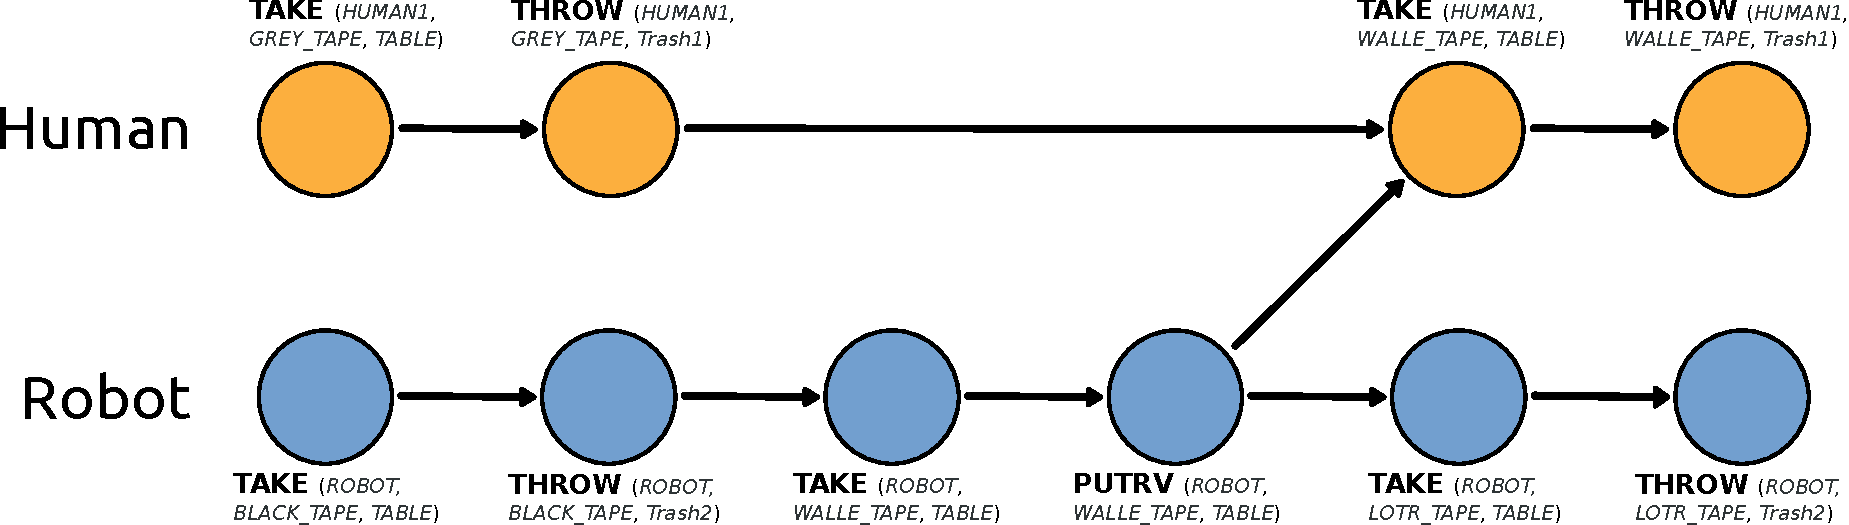
\includegraphics[width=0.95\columnwidth]{./figs/first_plan.pdf}
  \caption{A plan produced by HATP with 2 streams}
  \label{plan_hatp1}
\end{figure}

\paragraph{Action costs and social rules}
A cost and a duration function is associated to each action.
The duration function provides a duration interval for the action
achievement and is used, in one hand, to schedule the different
streams and, in the other hand, as an additional cost function.
In addition to these costs, HATP also takes into account a set of social
rules.  Social rules are constraints aiming at leading the plan
construction towards the best plan according to some human
preferences. The social rules we have defined so far deal with:

\begin{itemize}
\item undesirable state: to avoid a state in which the human could
  feel uncomfortable;
\item undesirable sequence: to eliminate sequences of actions that can
  be misinterpreted by the human;
\item effort balancing: to adjust the work effort of the agents;
\item wasted time: used to avoid long delays between the actions of
  the human partner;
\item intricate links: to limit dependencies between the actions of
  two or more agents.
\end{itemize}

\begin{figure}[htbp]
  \centering
  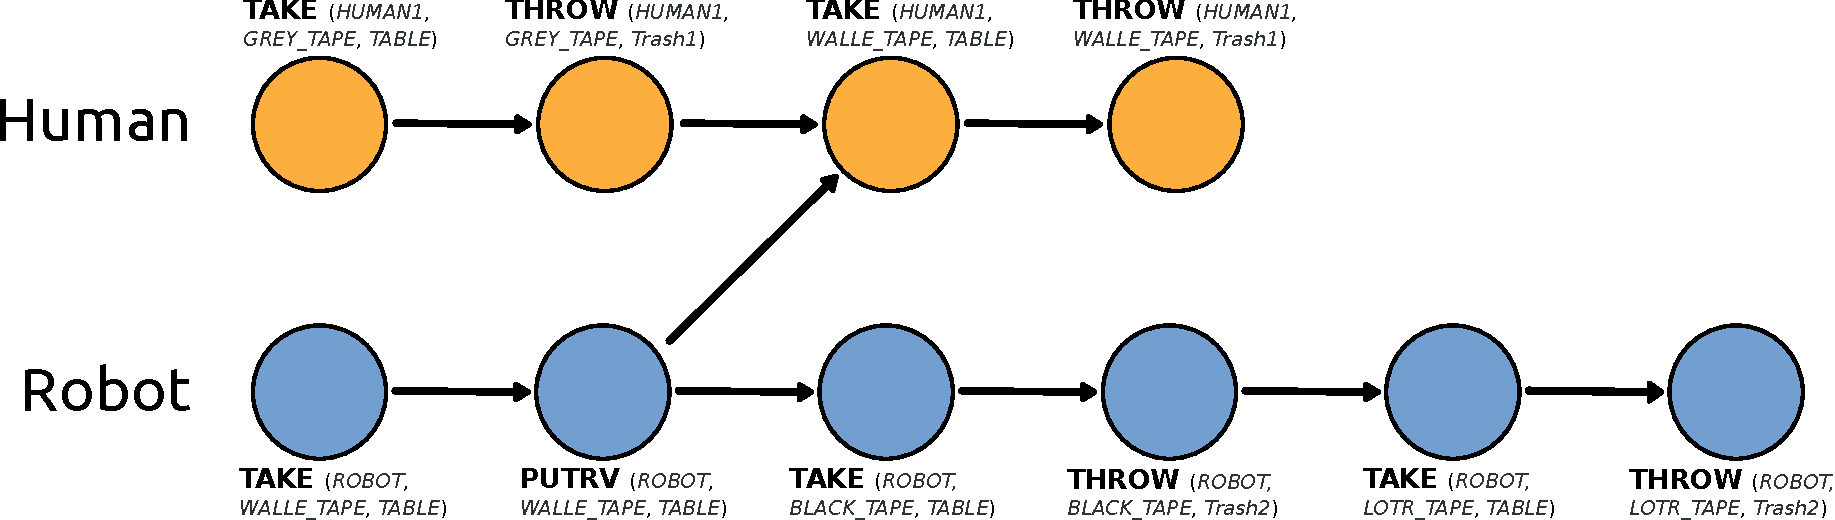
\includegraphics[width=0.95\columnwidth]{./figs/second_plan.pdf}
  \caption{A plan with the wasted time social rule}
  \label{plan_hatp2}
\end{figure}

Figure~\ref{plan_hatp2} illustrates an alternative plan to the previous 
one (Figure~\ref{plan_hatp1}) if the wasted time social rule is used.
The obtained shared plan is the best plan according to a global evaluation of
these multiple criteria.

\fxwarning{Relate HATP social rules to other AI techniques}

\paragraph{Several levels of cooperation} 
By tuning its costs
and adapting its social rules, HATP can be used to compute various
alternative plans. These plans can be categorized into several levels
of cooperation

\begin{itemize}
\item helping the human to achieve his goal by acting for him
\item sharing concrete resources by handing some objects
\item collaboration of the robot and the human by coordinating their
  actions towards a human-robot joint goal.
\end{itemize}



Two important remarks: because HATP is a generic symbolic task planner, we have
been able to design a planning domain at a semantic level which is close to the
one used in the human-robot dialogue (the planner vocabulary contains concepts
like \texttt{give}, \texttt{table}, \texttt{is on}...). Hence only a few
ontology rules have been required to map both the knowledge extracted from the
situation assessment and the statements originated from the verbal interaction
to the planner domain.

Second remark, after some research (see appendix B of~\cite{Lemaignan2012a} for
a detailed discussion)  we have decided to represent neither the planning
domain nor the resulting plans in the knowledge base: the planning domain (with
task pre- and postconditions) is stored in a specific format, outside of the
central declarative knowledge repository, and the plans are directly
communicated to the robot controller. Thus, like many other cognitive
architectures, we have independent declarative and procedural knowledge stores.


%%%%%%%%%%%%%%%%%%%%%%%%%%%%%%%%%%%%%%%%%%%%%%%%%%%%%%%%%%%%%%%%%%%%%%%%%%%%%%%%
\subsection{Robot control}
\label{sect|ctrl}

\subsubsection{Desires and experiences}

Our robot execution controllers (OpenPRS-based {\sc Shary} or Python-based {\sc
pyRobots}) have deep integration with the knowledge base. It serves as the
primary source of information for semantic-aware decision-making.

We split the interaction situations stemming from the situation assessment and
communication components in two categories: \emph{desires} (performative act)
and \emph{experiences} (assertive act).

\emph{Desires} are typically human orders (``Give me that book''). The nature
of the desired action (to pick, give, look, bring, show...), along with the
action parametrization (what is acted on? who should perform the action? etc.)
are extracted from the knowledge base, and either passed to a task planner
(presented in the next section) or executed if the procedure is directly
available.

\emph{Experiences}, on the other hand, comprise of emotions, states and
questions (when asking a question, we consider the human to be in an
\emph{interrogative state}). When the knowledge base recognizes that an agent
\emph{experiences} a particular emotion or state, the execution controller may
decide to handle it, typically by trying to answer the question or using the
emotional or physical state as a parameter for subsequent actions. As an example,
when the speaker says ``I feel tired'', we change the motion planner
parametrization to lower the effort the human needs to provide for the following
joint manipulation tasks. Note that this example has been implemented as a
proof-of-concept. We have not yet tried to define a theoretical framework that
would support action alteration based on the user's experienced states.

\subsubsection{Event-driven control}

The {\sc Oro} server proposes two paradigms to access its content: RPC-style
queries (based on the standard SPARQL language) or events. In its simplest
form, a module can subscribe to an event by passing through an event pattern
(in its basic form, a partial statement like \stmt{? type Elephant}) and a
callback.  Each time a new instance of elephant appears in the knowledge base,
the callback is triggered.

This allows us to write reactive robot controllers with a high level of
expressiveness: for instance, by subscribing to the event \stmt{human1 desires
?action, ?action type Look, ?action hasGoal myself}, we could trigger a
behaviour when the human expresses (through dialogue, gestures...) that he
wants to look at the robot itself.

The robot controller designer does not need to directly care about how this
\emph{desire} is produced (this is delegated to perception modules), he can
focus on the semantic of the desire.

Note also that we take advantage of the reasoning capabilities of the system:
for example, the goal of the action (\stmt{action hasGoal myself}) may not be
explicitly asserted, but inferred by the reasoner based on other assertions.

\subsubsection{Action execution and monitoring}\label{sec:action}

The action execution and monitoring task involves the motion and task
planning, the effectors and the dedicated robot controller activity
(Figure~\ref{architecture_fg}).


\paragraph{Human aware motion, placement and manipulation planning}
In our scenarios, actions are only object manipulation actions: Pick,
Place, Throw, Give. Motion and Task planning allows to compute final
object placement, grasp and arm motion trajectories taking into
account task specific constraints and human postures, abilities and
preferences: see \cite{Sisbot2008, Mainprice2011, Pandey2010} for
details.


\paragraph{Action Execution and Monitoring Robot Controller}
context and on the shared plan elaborated by HATP for a given goal,
the robot controller decides to execute an action or to ask its human
partner to do it.  Actions feasibility by the human or the robot are
regularly reconsidered based on the reachability / visibility
computation mechanisms.

Robot action execution is based on simple automatons  that translate
symbolic planning atomic actions into sequences of planned arm motions
and gripper commands to execute according to current state
of the 3-tuple (gripper, object, furniture). We have three states
according to whether the object is in gripper and if it is in gripper
whether it is on furniture.  These states are directly obtained from
the updated symbolic state of the world in the ontology.

For plan action monitoring, primitive actions recognition defined
above are used. A primitive action detection is interpreted as action
success if it is the expected one and failure otherwise. The robot
also reacts to the absence of activity.









%%%%%%%%%%%%%%%%%%%%%%%%%%%%%%%%%%%%%%%%%%%%%%%%%%%%%%%%%%%%%%%%%%%%%%%%%%%%%%%%
%%%%%%%%%%%%%%%%%%%%%%%%%%%%%%%%%%%%%%%%%%%%%%%%%%%%%%%%%%%%%%%%%%%%%%%%%%%%%%%%
%%%%%%%%%%%%%%%%%%%%%%%%%%%%%%%%%%%%%%%%%%%%%%%%%%%%%%%%%%%%%%%%%%%%%%%%%%%%%%%%

\section{Experimental results}

\fxfatal{Most of the Experiment section needs to be written}

We assume here that the robot (and the human) has been given the joint goal
``CLEAN TABLE''. For HATP, this means putting all tapes that are
currently on the table in the trashbin. Depending on the state of the
world and agent preferences, different plans are produced.

Figure~\ref{plan-etat2} shows a plan produced to clean the table based on the initial the initial state given in  \S~\ref{sub:gtrc}.

\begin{figure*}[thpb]
  \centering
  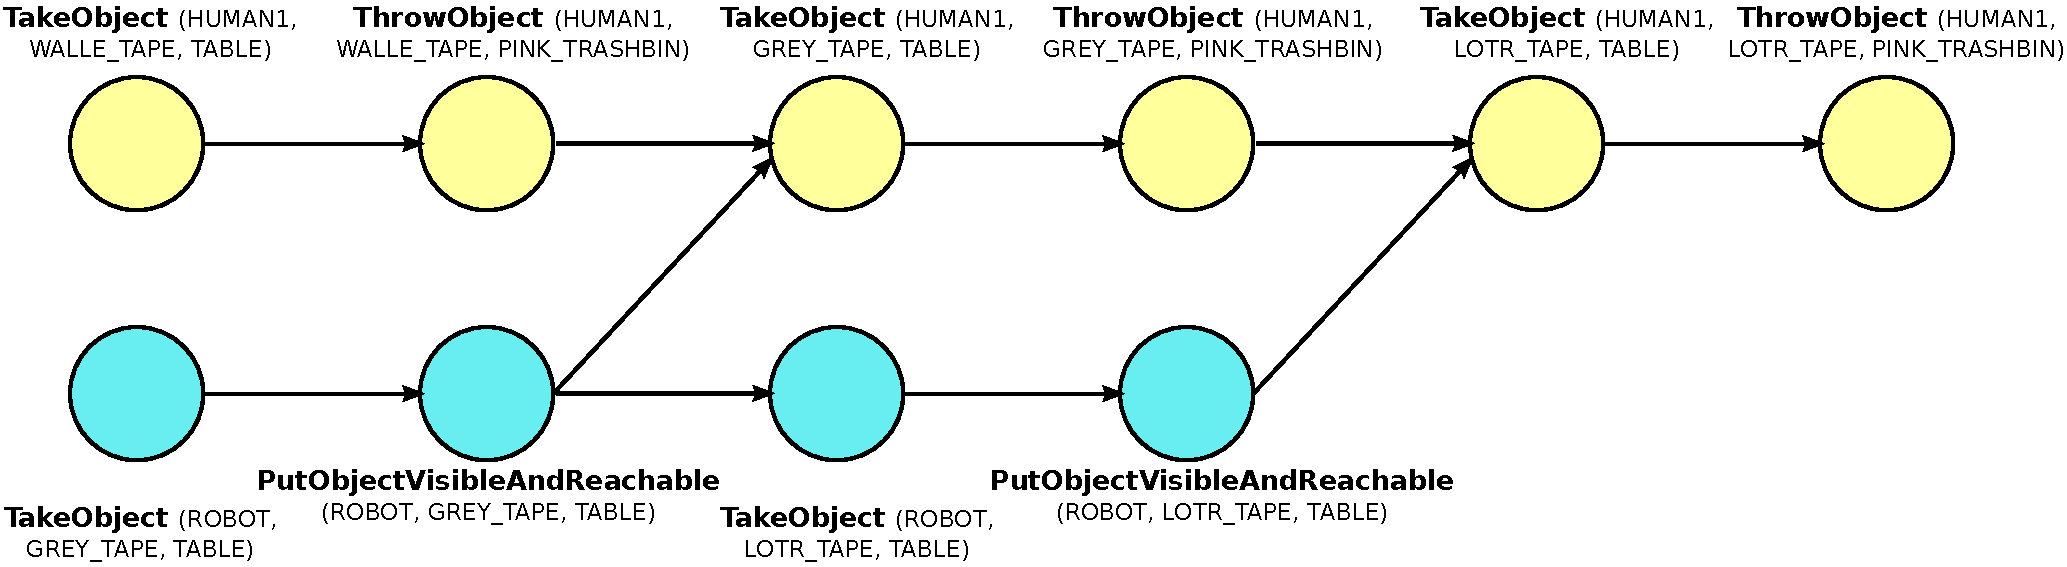
\includegraphics[width=1.0\textwidth]{./figs/plan3.pdf} \\
  \caption {A plan produced by HATP for clean the table based on the initial state given in \S~\ref{sub:gtrc}}
  \label{plan-etat2}
\end{figure*}

Let us now take a simpler example to illustrate a full run of the
system. We have only one tape on the table and it is is reachable only
by the robot while the throw position on top of the trashbin is
reachable only by the human.

\begin{figure*}[thpb]
  \centering
    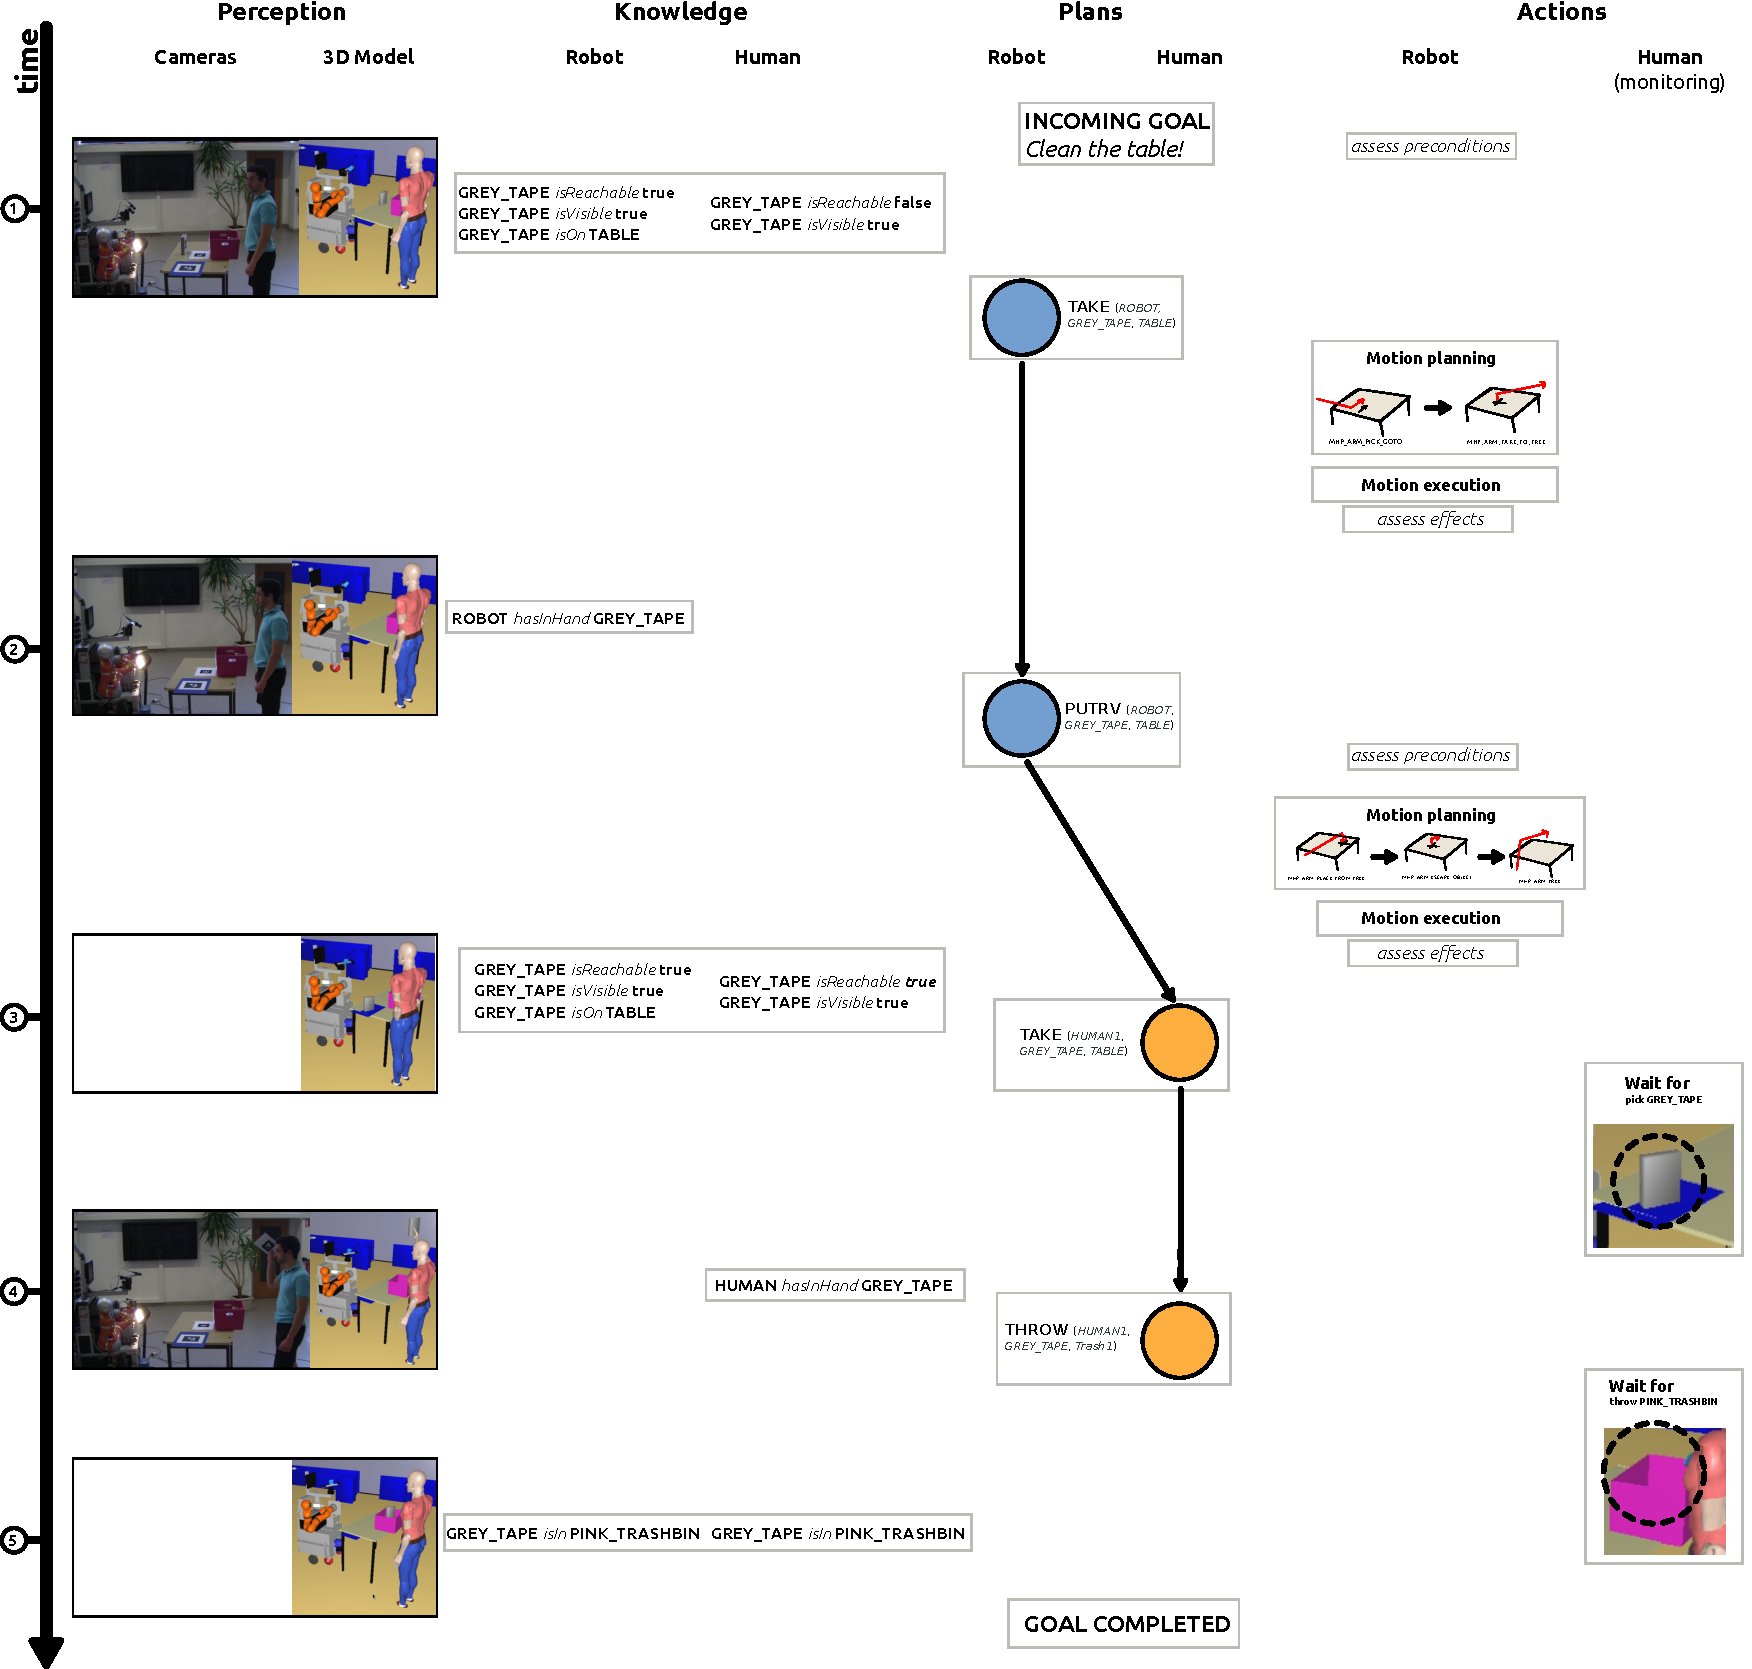
\includegraphics[width=1.0\textwidth]{./figs/manip_run.pdf} \\
    \begin{center}
    \caption {An example of a human-robot collaborative goal achievement}
    \end{center}
  \label{manip_run_fg}
\end{figure*}


%\subsection{successful execution}

Figure~\ref{manip_run_fg} illustrates the main processes occurring
during a multi-step human-robot collaborative goal achievement.  The
plan produced is quite straightforward and is shown in the third row
called ``Goal and Plan''. It consists in 4 successive actions
involving the robot and the human. Robot grasps the tape and then
places it on the table at a position where it is visible and reachable
for the human. Human then is asked to pick the tape and throw it in
the trashbin. The first row, named ``Cameras'', shows several
snapshots corresponding to various execution steps. Snapshot~1
presents the initial situation. Snapshots~2, 3, 4 and 5 give the state
after the successive achievement of the four actions in the plan. The
second row, named ``3D Model'', shows the display of SPARK at the same
instants. The fourth, row called ``Robot Speech Acts'', gives robot
speech acts produced along the execution to inform the human partner
about goal and plan creation and status and to verbalize the actions
that the human is asked to execute. The fifth row illustrates robot
knowledge on itself and on the objects. The sixth row illustrates the
robot knowledge about the human state. The seventh row gives ongoing
robot action with action preconditions and effects assessment as well
as motion execution tasks. Motion trajectory typology can be found
between the 3D Model views. The eighth row gives ongoing human action
with action preconditions and effects assessment and monitoring
activity.


%%%%%%%%%%%%%%%%%%%%%%%%%%%%%%%%%%%%%%%%%%%%%%%%%%%%%%%%%%%%%%%%%%%%%%%%%%%%%%%%
%%%%%%%%%%%%%%%%%%%%%%%%%%%%%%%%%%%%%%%%%%%%%%%%%%%%%%%%%%%%%%%%%%%%%%%%%%%%%%%%
%%%%%%%%%%%%%%%%%%%%%%%%%%%%%%%%%%%%%%%%%%%%%%%%%%%%%%%%%%%%%%%%%%%%%%%%%%%%%%%%

\section{Perspectives}
\label{sect|conclusion}

\subsection{Contributions and Related work}\label{sec:soa}

The human presence brings new requirements for robot's abilities both
at the functional and at the deliberative levels~\cite{Klein2004}. The
topics involve motion~\cite{Kulic2007,Berg2004,Madhav2006},
navigation~\cite{Althaus2004,Sisbot2007}, manipulation~\cite{Kemp2007}
in presence of humans as well as perception of human
activities~\cite{Breazeal2001,Burger2008}. Also, when
interacting with humans, robots need to incorporate communication and
collaboration abilities. Several theories dealing with
collaboration~\cite{Cohen1991,Grosz1996,Clark1996} emphasize that
collaborative tasks have specific requirements compared to individual
ones, \eg, since the robot and the person share a common goal, they
have to agree on the manner to realize it, they must show their
commitment to the goal during execution, etc. Several robotic systems
have already been built based on these
theories~\cite{Rich1997,Sidner2005,Tambe2005a,Breazeal2003} and they
all have shown benefits of this approach. They have also shown how
difficult it is to manage turn-taking between communication partners
and to interleave task realization and communication in a generic
way. Finally, today only few
systems~\cite{Fong_2006,Breazeal2003,Sisbot2008} take humans into
account at all levels.

Perspective Taking is a human ability which allows one to put
him/herself in another person's point of view. Studied in
psychology literature~\cite{Flavell1992,Tversky1999}, this ability is
crucial when interacting with people by allowing one to reason on
others' understanding of the world in terms of visual perception, spatial
descriptions, affordances and beliefs, etc.
Therefore, in the last years these notions have been gradually
employed in Human-Robot Interaction.~\cite{Breazeal2006} presents a
learning algorithm that takes into account information about a
teacher's visual perspective in order to learn a
task. ~\cite{Johnson2005} apply visual perspective taking for action
recognition between two robots.~\cite{Trafton2005} use both visual and
spatial perspective taking for finding out the referent indicated by a
human partner.

Spatial reasoning~\cite{O'Keefe1999}, on the other hand, has been used
for natural language processing for applications such as direction
recognition ~\cite{Kollar2010,Matuszek2010} or language
grounding~\cite{Tellex2010}.~\cite{Skubic2004} presented a spatial
reasoner integrated in a robot which computes symbolic positions of
objects.

\subsection{Knowledge-oriented architecture}

Altogether, the components we have presented compose an architecture that we
call \emph{knowledge-oriented}:

\begin{itemize}
    
    \item{Knowledge is explicitly stored in one central and consistent
    repository of facts, accessible for all modules.} 

    \item{Knowledge is represented in a strict formalism (OWL statements) and
    with a clearly defined vocabulary (stated in the common-sense ontology).}

    \item{The first two points enable a loosely-coupled architecture where
    modules can be removed or replaced easily by other ones as long as
    they share the same semantics (modules are defined by the knowledge they
    produce),} 

    \item{We adopt a \emph{symbolic}, reactive, event-driven approach to robot control.
    By managing events at the same level as the reasoner, we take full
    advantage of the inference abilities of {\sc Oro} to trigger events whose
    \texttt{true} conditions can be inferred.} 

    \item{Finally, this architecture allows for the combination of very
    different knowledge modalities in a single homogeneous environment,
    bringing mutual benefits to components. For instance, the dialogue
    processing module can perfectly run without any geometric
    perception, but its disambiguation routines can transparently
    benefit from it when available (since richer symbolic descriptions of
    objects are then available).}

\end{itemize}

Those items are not new \emph{per se}. It seems however interesting to
underline the shift of focus this implies during the design and integration
phases. 

\fxfatal{Insert here discussion of other major KRR systems for robots (Severin)}

\subsection{The Next Steps}


In this paper we have presented a decisional framework designed for
robots operating in a human environment. Our objective is to provide a
management of human-robot interaction that is an integral part of a
general robot control architecture.  This was done in order to provide
a principled way to deal with HRI scenario.  The framework is also
suitable for the development and experiment of task planners and
interaction schemes that explicitly consider human abilities and
preferences.

The design choices and the results presented here are still preliminary.
While the general scheme we propose might be difficult to implement in
a general sense, we believe that it is a reasonable challenge to
implement it in the case of a personal robot assistant essentially
devoted to fetch-and-carry, as well as for interactive manipulation
tasks and associated activities.



\section*{Acknowledgment}

This work has been supported by EU FP7 ``SAPHARI'' under grant agreement no. ICT-287513.

\bibliographystyle{elsarticle-num}
%\bibliographystyle{abbrv}
\bibliography{laas_hri}



\end{document}
